\documentclass{article}
\usepackage[utf8]{inputenc}
\usepackage{graphicx}
\usepackage{listings}
\usepackage{mathtools}
\usepackage{geometry}
\usepackage{amsmath}
\usepackage{wrapfig}
\usepackage{float}
\usepackage{subcaption}
\usepackage{tabularx}
 \geometry{
 a4paper,
 total={175mm,257mm},
 left=20mm,
 top=20mm,
 }
\title{Homework-6}
\author{Susan Sapkota and Anish Adhikari}

\date{November 2020}

\begin{document}

\maketitle

\section{Introduction}
Scientific Computational problem most of time involves lot of calculation which takes time longer time to solve numerically in normal laptop or computer. The Equations like Einstein field equation in certain condition takes around 10 to 100 years to find solution. We can technically solve same problem in less time by using the divide and conquer technique in programming knows as Parallel computing.

Parallel computing is simultaneous use of multiple processors to solve scientific problem given that problem can be broken into discrete pieces which can solved simultaneously in less time. In nature, Many complicated events are happening at same time like supernova explosion, merging of black hole within temporal sequence. In this Project, we use parallel computing technique i.e openMP to resolve homework-4 and compare computing time using stampede2 supercomputer. 

\section{OpenMP}
OpenMP or Open Multiprocessing is application programming Interface that supports C/C++ and Fortran which is designed for multi-processing and shared memory. Shared memory is computer architecture where all processors have direct access to main memory and work independently as unit. openMP uses threads, which is the smallest unit of supercomputer to execute task prompted by operating system.We can run program in multiple thread to run it parallel , and we can control all the threads using fork-joint model.
\subsection{Speedup and Efficiency}

We can define the parallel speed up deoted by S as :-
\begin{equation}
     S= \frac{T_s}{T_p}  \leq \frac{1}{1-P}
\end{equation}
     Where $T_{s}$ is the serial run time and $T_{p}$ is the parallel run time and P is the fraction of code that can be run Parallel and $P\in[0,1]$\newline
     
  The above equation is also known as Amdahl's  Law.The value of P is depends on how much of the code can be paralyzed The value of P will equals 0 if the code can't be parallelized the parallel speed up equals 1. The parallel speed up will be infinite if all the code can be parallelized and P=1.
   If we use run the code on multiple processor then that does not necessarily mean that the computing time will he halved.Suppose half the code can be parallelized  then with Amdhal's law the parallel speed up will be 2 and if the 60 percent of the code can be parallelized then the speed up will be 2.5 meaning that the run time will be 2 and 2.5 times faster when 50 and 60 percent of code are parallized  but the remaining 50 percent and 40 percent will have to be run in a sequential runtime  and will still take half of the time. If we parallized 100 percent of the code then the Parallel speed up will be reduced to zero which is not possible. So, it will still take time.
  
  Let us consider our parallel machine system has $N_p$ processors. Then we have,
  \begin{equation}
      T_p \leq (1-P) T_s + P \frac{T_s}{N_p}
  \end{equation}
  For the best case, we can consider equality. when the number of processor increases then second right term vanishes and we have 
  \begin{equation}
        \lim_{N_p \to +\infty} T_p =  \frac{T_s}{S}
  \end{equation}

Efficiency is defined as effectiveness of system in transforming the input into output with number of cores. Let S be speed up and efficiency(E) is given by,
\begin{equation}
    E = \frac{S}{N_p}
\end{equation}

\subsection{Scalability}
Scalability is defined as ability of parallel system to  demonstrate a proportional increase in parallel speedup with more resources. we have two types of scaling as weak and strong. for strong scaling we have to check how does the program or algorithm perform when we increases number of parallel processor for fixed problem? The main aim is to run same problem scale faster. In theory, Perfect scaling means problem is done in $\frac{1}{N_p}$ time then in serial time. For weak scaling, we have to check how does our program or algorithm performs when we increase problem size N with increasing number of processor$N_p$? The aim of weak scaling is to run larger problem in same time. in the case of central difference and 2D trapezoidal, the error is 2nd order. So, on increasing the core we have to increase the problem size by $\sqrt{N_p}$. 


\subsection{Stampede2}
For our project we will be using the super computer named stampede2 located at University of Austin at Texas. This supercomputer consist of 4200 nodes (processors) each of this node has 68 cores and each core consist of 4 threads. Thread is smallest unit of the core that can each execute a 1 or more sets of instructions.

 \section{Design of Parallel Program}
We used shared memory (openMP) to build parallel program that can differentiate and integrate the first combination of homework-4. we have function $u(x,y)=sin(x) cos(y)$ and the mapping $x(r,s)=r+0.1s$ and $y(r,s)=s$ in $(x,y)\in\Omega$ and $(r,s)\in\Omega_R=[-1,1]^2$. For simplicity, we set the number of grid in both direction $\Omega_R$ is same. i.e. $n_r=n_s=n$ with $h_r=h_s=\frac{2}{n}$.$u_x$ and $u_y$ is computed using 2nd order finite difference. The error is given by,
\begin{align}
    & \text{err}(h_r, h_s)
        = \left|
            \int_{\Omega}
                \left(
                    u_x(x, y) + u_y(x, y) -
                        \big[
                            (u_\text{exact})_x(x, y) + (u_\text{exact})_y(x, y)
                        \big]
                \right)^2
                \, dx dy \right|^{\tfrac{1}{2}} 
\end{align}
        where $h_r$ and $h_s$ are the step sizes. The effective grid-size is $h_{eff}=\sqrt{h_r h_s maxJ}$. Note  $(u_\text{exact})_x(x, y)= cos(x) cos(y)$ and $(u_\text{exact})_y(x, y)=-sin(x) sin(y)$.

We did domain decomposition in order to make our large code into discrete chunk of work. we discretize the grid into n points and h step-size. We call OMP\_set\_num\_threads() to set the number of core use in processing. we then use OMP PARALLEL DO PRIVATE to parallel our program to compute grid point r,s,x and y, function $u(x,y)$, $u_r$,$u_s$,$x_r$,$x_s$,$y_r$ and $y_s$. for example, if we used two processor with 200 grid size then each processor compute above function for 100 grid. we didn't parallelize the code to compute metric or jacobian. Then we used OMP WORKSHARE to compute $u_x$, $u_y$ and function inside of error equation-5.finally,we used 2D trapezoidal rule to compute error. So, we parallelize our code around 70-80 percent.   
\section{Results and Discussion}
We calculated error (equation-5) using homework-4 code. The error does converge according to $O(h^2)$ shown in figure 1. Then we paralleled our code using section 3 and calculated error. The below table show the error run in 1-8 core in stempede2 and error does converge according to  $O(h^2)$.

\begin{tabularx}{0.8\textwidth} { 
  | >{\raggedright\arraybackslash}X 
  | >{\centering\arraybackslash}X 
  | >{\raggedleft\arraybackslash}X | }
 \hline
 Number of core & Error \\
 \hline
 1  & 3.9945559168467637E-005 \\
\hline
\hline
 2  & 3.9945559168467637E-005 \\
\hline
\hline
 3  & 3.9945559168467637E-005  \\
\hline
\hline
 4  & 3.9945559168467637E-005 \\
\hline
\hline
 5  & 3.9945559168467637E-005 \\
\hline
\hline
 6  & 3.9945559168467637E-005 \\
\hline
\hline
 7  & 3.9945559168467637E-005  \\
\hline\hline
 8  & 3.9945559168467637E-005  \\
\hline
\end{tabularx}

So, calculation of error remains same irrespective of number of cores used. 
\newline

The size of problem is fixed for strong scaling with increasing number of cores(1-16). In theory, we expect the parallel time decreases with $\frac{1}{N_p}$ with increasing $N_p$. We do see in figure 2(a) when we increasing the cores parallel time is not decreasing with our expectation might be due to small size of problem and communication cost between cores. When we increase the size of problem to 2000-2000 grid the timing decreasing rapidly might be each core get enough number of grid to compute. The graph 2(c) and 2(d) is about speed up with increasing node. Initially, The speed increase rapidly for 20 grid size when we increase the number of core but it get flattened on further increasing core as the problem size is small so not effective to used many core due to communication cost. The interesting one is for the grid 800, it speed up little and try to flattened soon. when the problem size is 2000 then on increasing core it lesser speed than previous and it flattened on increasing core. Ideally, Efficiency of parallel system is horizontal line. For the small problem 20 grid size, initially the efficiency increase but decreases on increasing core as we are doing small task with multiple core might be due to load  imbalance and minimum concurrency on multiple processor. when increasing the problem size  800 and 2000, the efficiency decreases on increasing number of cores. The graphs might not be as expected (flat) due to the program not being fully parallelized like metric calculation and final error calculation.

For the weak scaling, the problem size increases with increasing the number of the processor used. We used (200,283,346,400,447,490,529,566,600,632,663,693,721,748,775,800) for the grid size for 1 to 16 core. Ideally, we expect the processing time to be linear. In the figure 3(a), we see the graph is almost linear with some irregularities because of partial parallelization of program. The parts which aren't parallelized might takes longer time due to overload of the data. The speed and efficiency also decrease with same reason rather than being flat.we can technically increase parallelization in our program to get more efficiency.

 \begin{figure}[!htb]
        \center{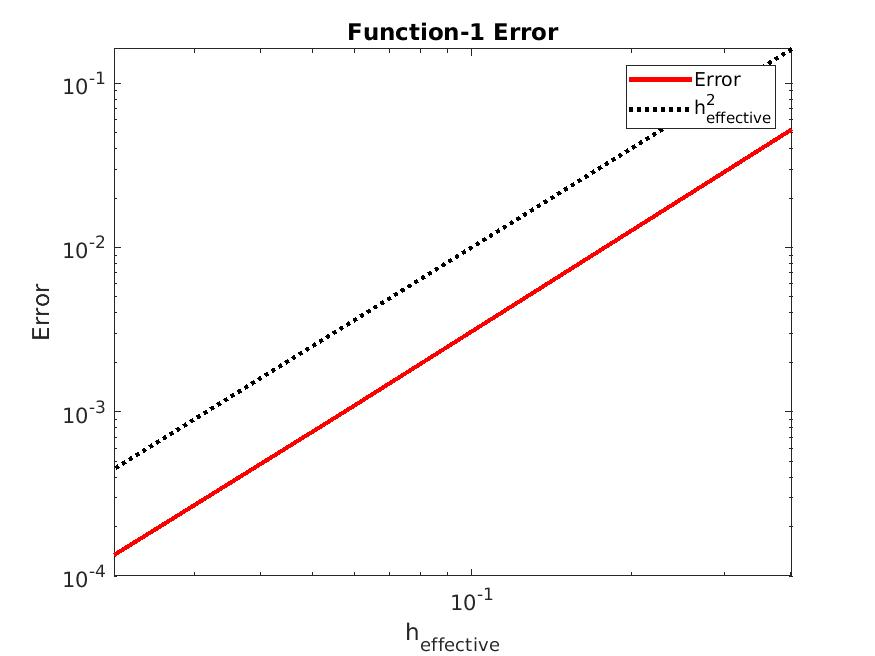
\includegraphics[width=\textwidth]{error-in-1.jpg}}
        \caption{\label{fig:my-label} Error vs Effective grid size}
      \end{figure}

\newpage

\begin{figure}[t!] % "[t!]" placement specifier just for this example
\begin{subfigure}{0.48\textwidth}
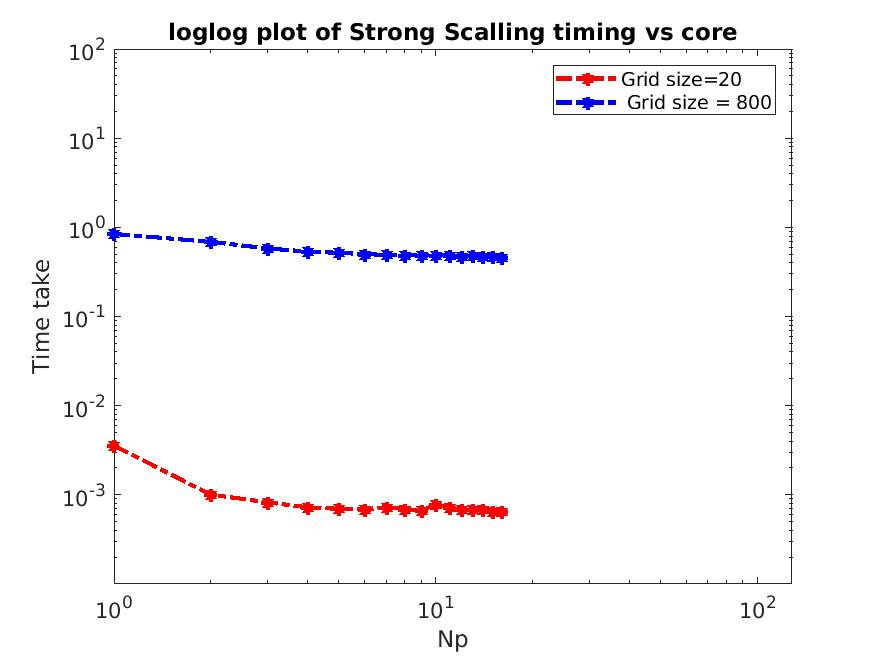
\includegraphics[width=\linewidth]{timing-strongscaling.jpeg}
\caption{Timing vs $N_p$} \label{fig:a}
\end{subfigure}\hspace*{\fill}
\begin{subfigure}{0.48\textwidth}
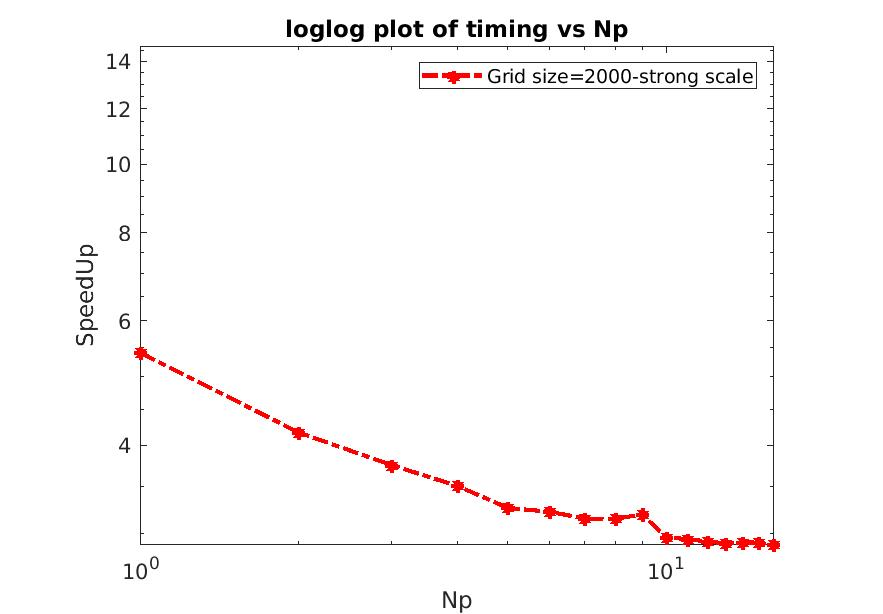
\includegraphics[width=\linewidth]{timing2000.jpeg}
\caption{Timing vs $N_p$} \label{fig:b}
\end{subfigure}

\medskip
\begin{subfigure}{0.48\textwidth}
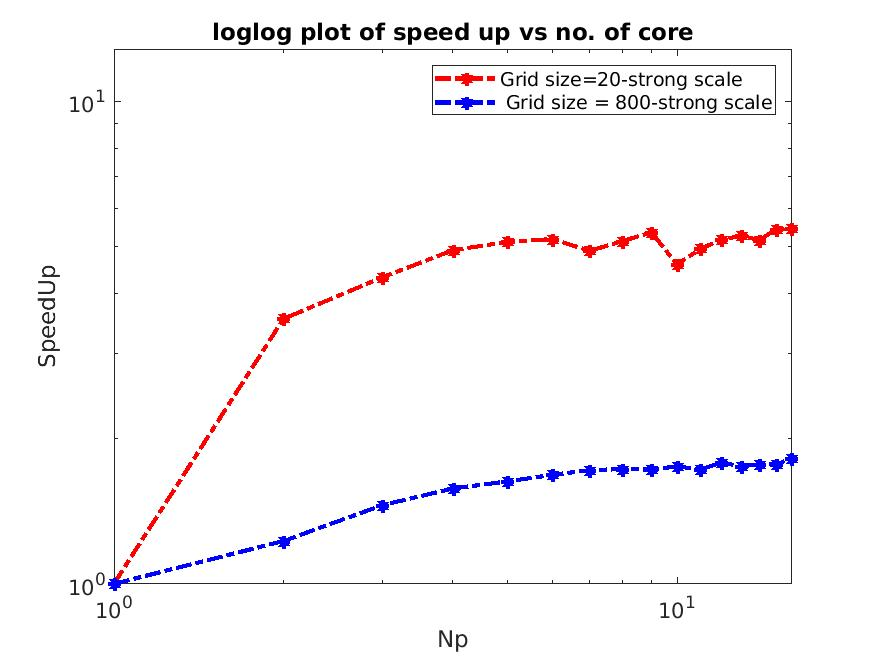
\includegraphics[width=\linewidth]{Speedupstrong.jpeg}
\caption{Speedup vs $N_p$ } \label{fig:c}
\end{subfigure}\hspace*{\fill}
\begin{subfigure}{0.48\textwidth}
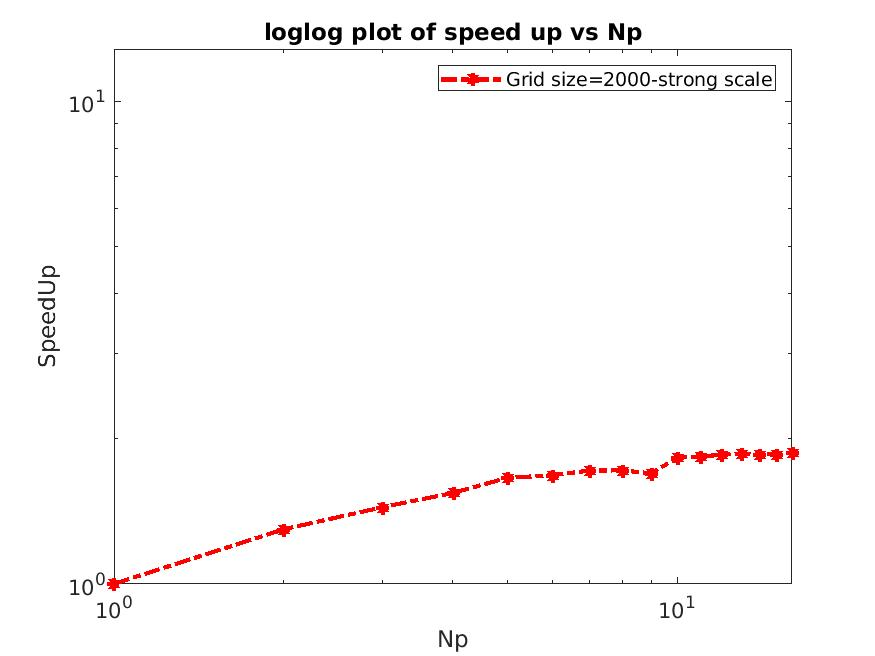
\includegraphics[width=\linewidth]{Speedup2000.jpeg}
\caption{Speedup vs $N_p$ } \label{fig:d}
\end{subfigure}

\medskip
\begin{subfigure}{0.48\textwidth}
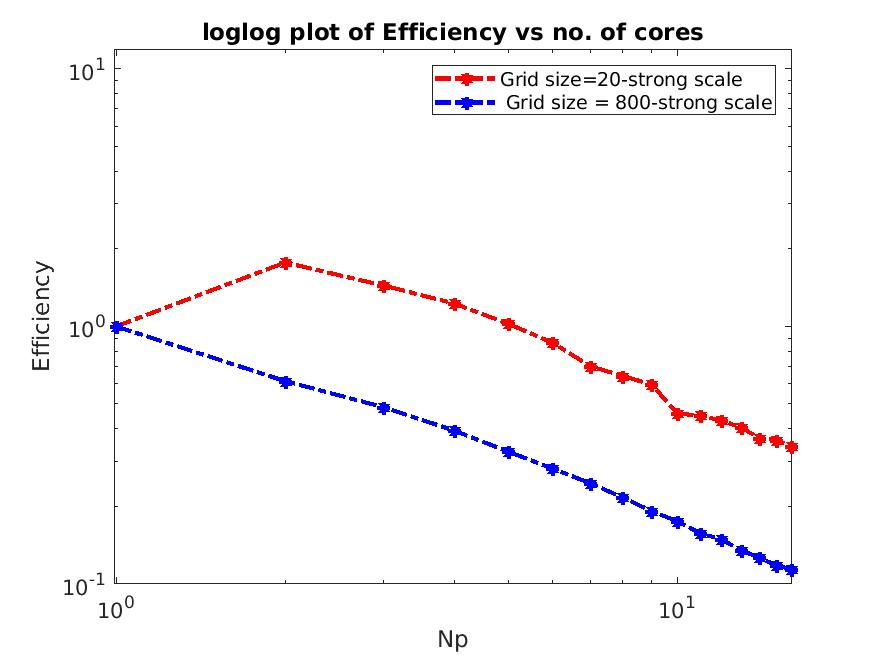
\includegraphics[width=\linewidth]{Efficiencystrong.jpeg}
\caption{Efficiency vs $N_p$ } \label{fig:e}
\end{subfigure}\hspace*{\fill}
\begin{subfigure}{0.48\textwidth}
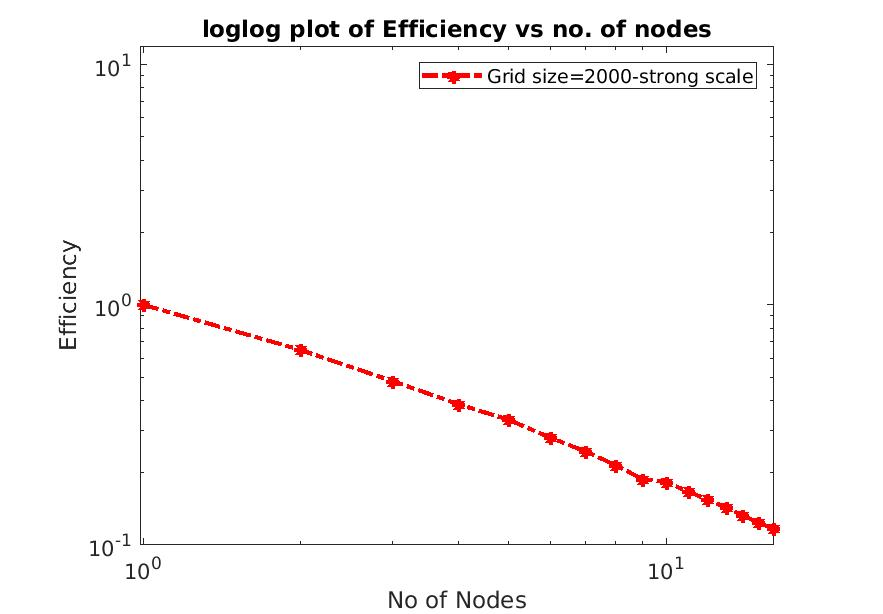
\includegraphics[width=\linewidth]{Efficiency2000.jpeg}
\caption{Efficiency vs $N_p$ } \label{fig:f}
\end{subfigure}

\caption{Strong Scaling} \label{fig:1}
\end{figure}

\newpage
\begin{figure}
    \begin{subfigure}{\textwidth}
    \centering
    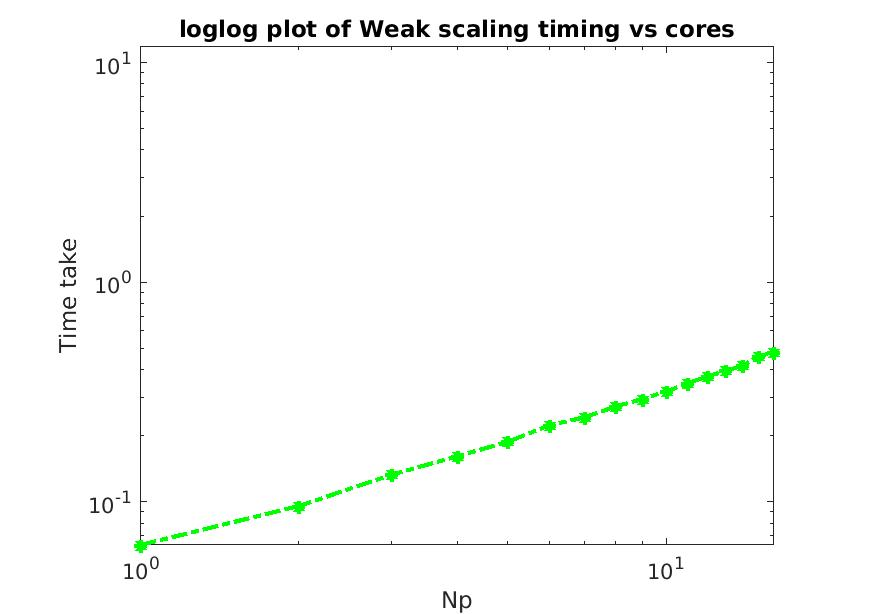
\includegraphics[scale=0.33]{timing-weakscaling.jpeg}
    \caption{Parallel time vs $N_p$}
    \label{fig:doc1}
    \end{subfigure}

    \bigskip
    \begin{subfigure}{\textwidth}
    \centering
    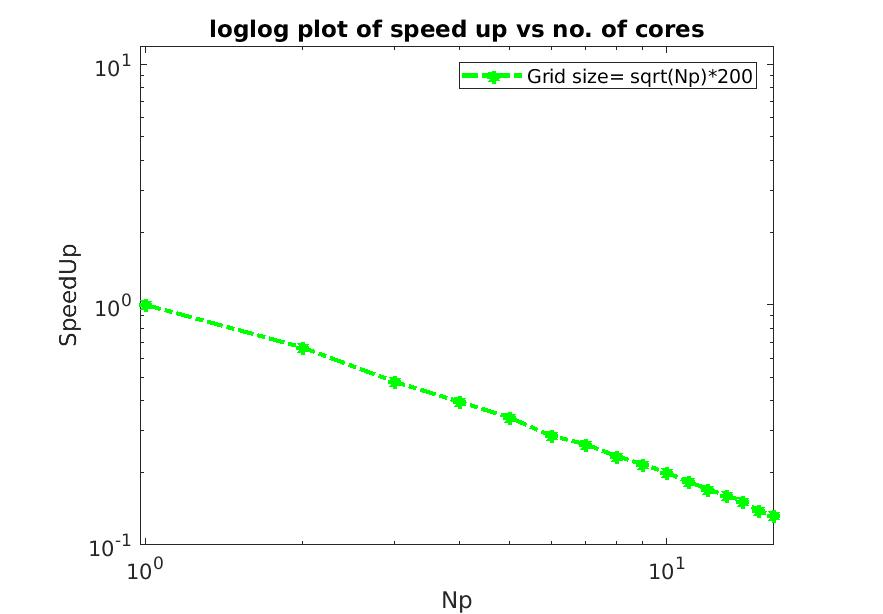
\includegraphics[scale=0.33]{Speedupweak.jpeg}
    \caption{Speedup vs $N_p$}
    \label{fig:doc2}
    \end{subfigure}
    \bigskip
    \begin{subfigure}{\textwidth}
    \centering
    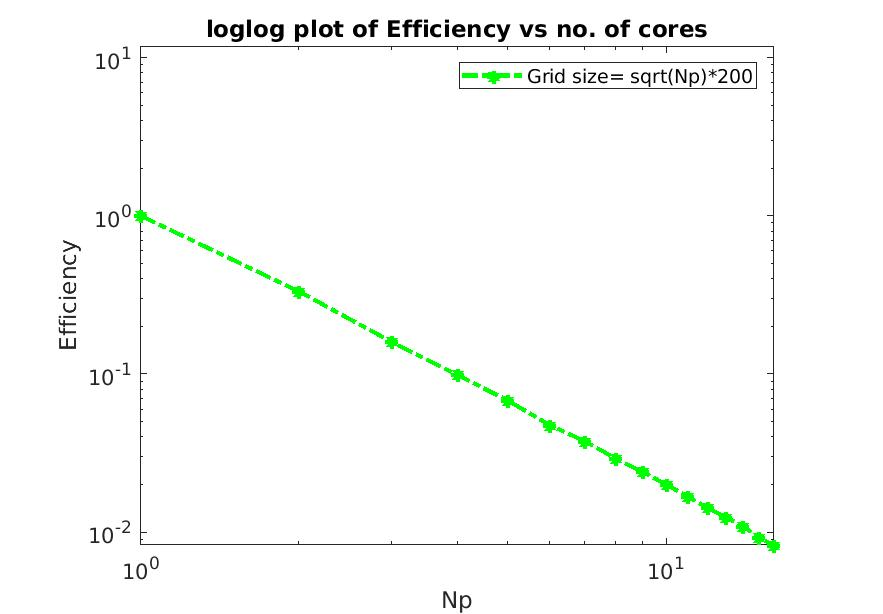
\includegraphics[scale=0.33]{Efficiencyweak.jpeg}
    \caption{Efficiency vs $N_p$}
    \label{fig:doc3}
    \end{subfigure}
    
\caption{Weak-Scalling}
\end{figure}



\end{document}

